\section{Results}

In this section, we summarise the results of our assessment. The descriptors considered in the evaluation are: BRISK, ORB, SURF and SIFT included in OpenCV library. The implementation of AKAZE made available by its original author \cite{alcantarilla13} and the implementation of SIFT using CUDA presented in \cite{bjorkmann14}.

\subsection{Distinctiveness}

%\begin{figure*}[t]
%\centerline{% 
%		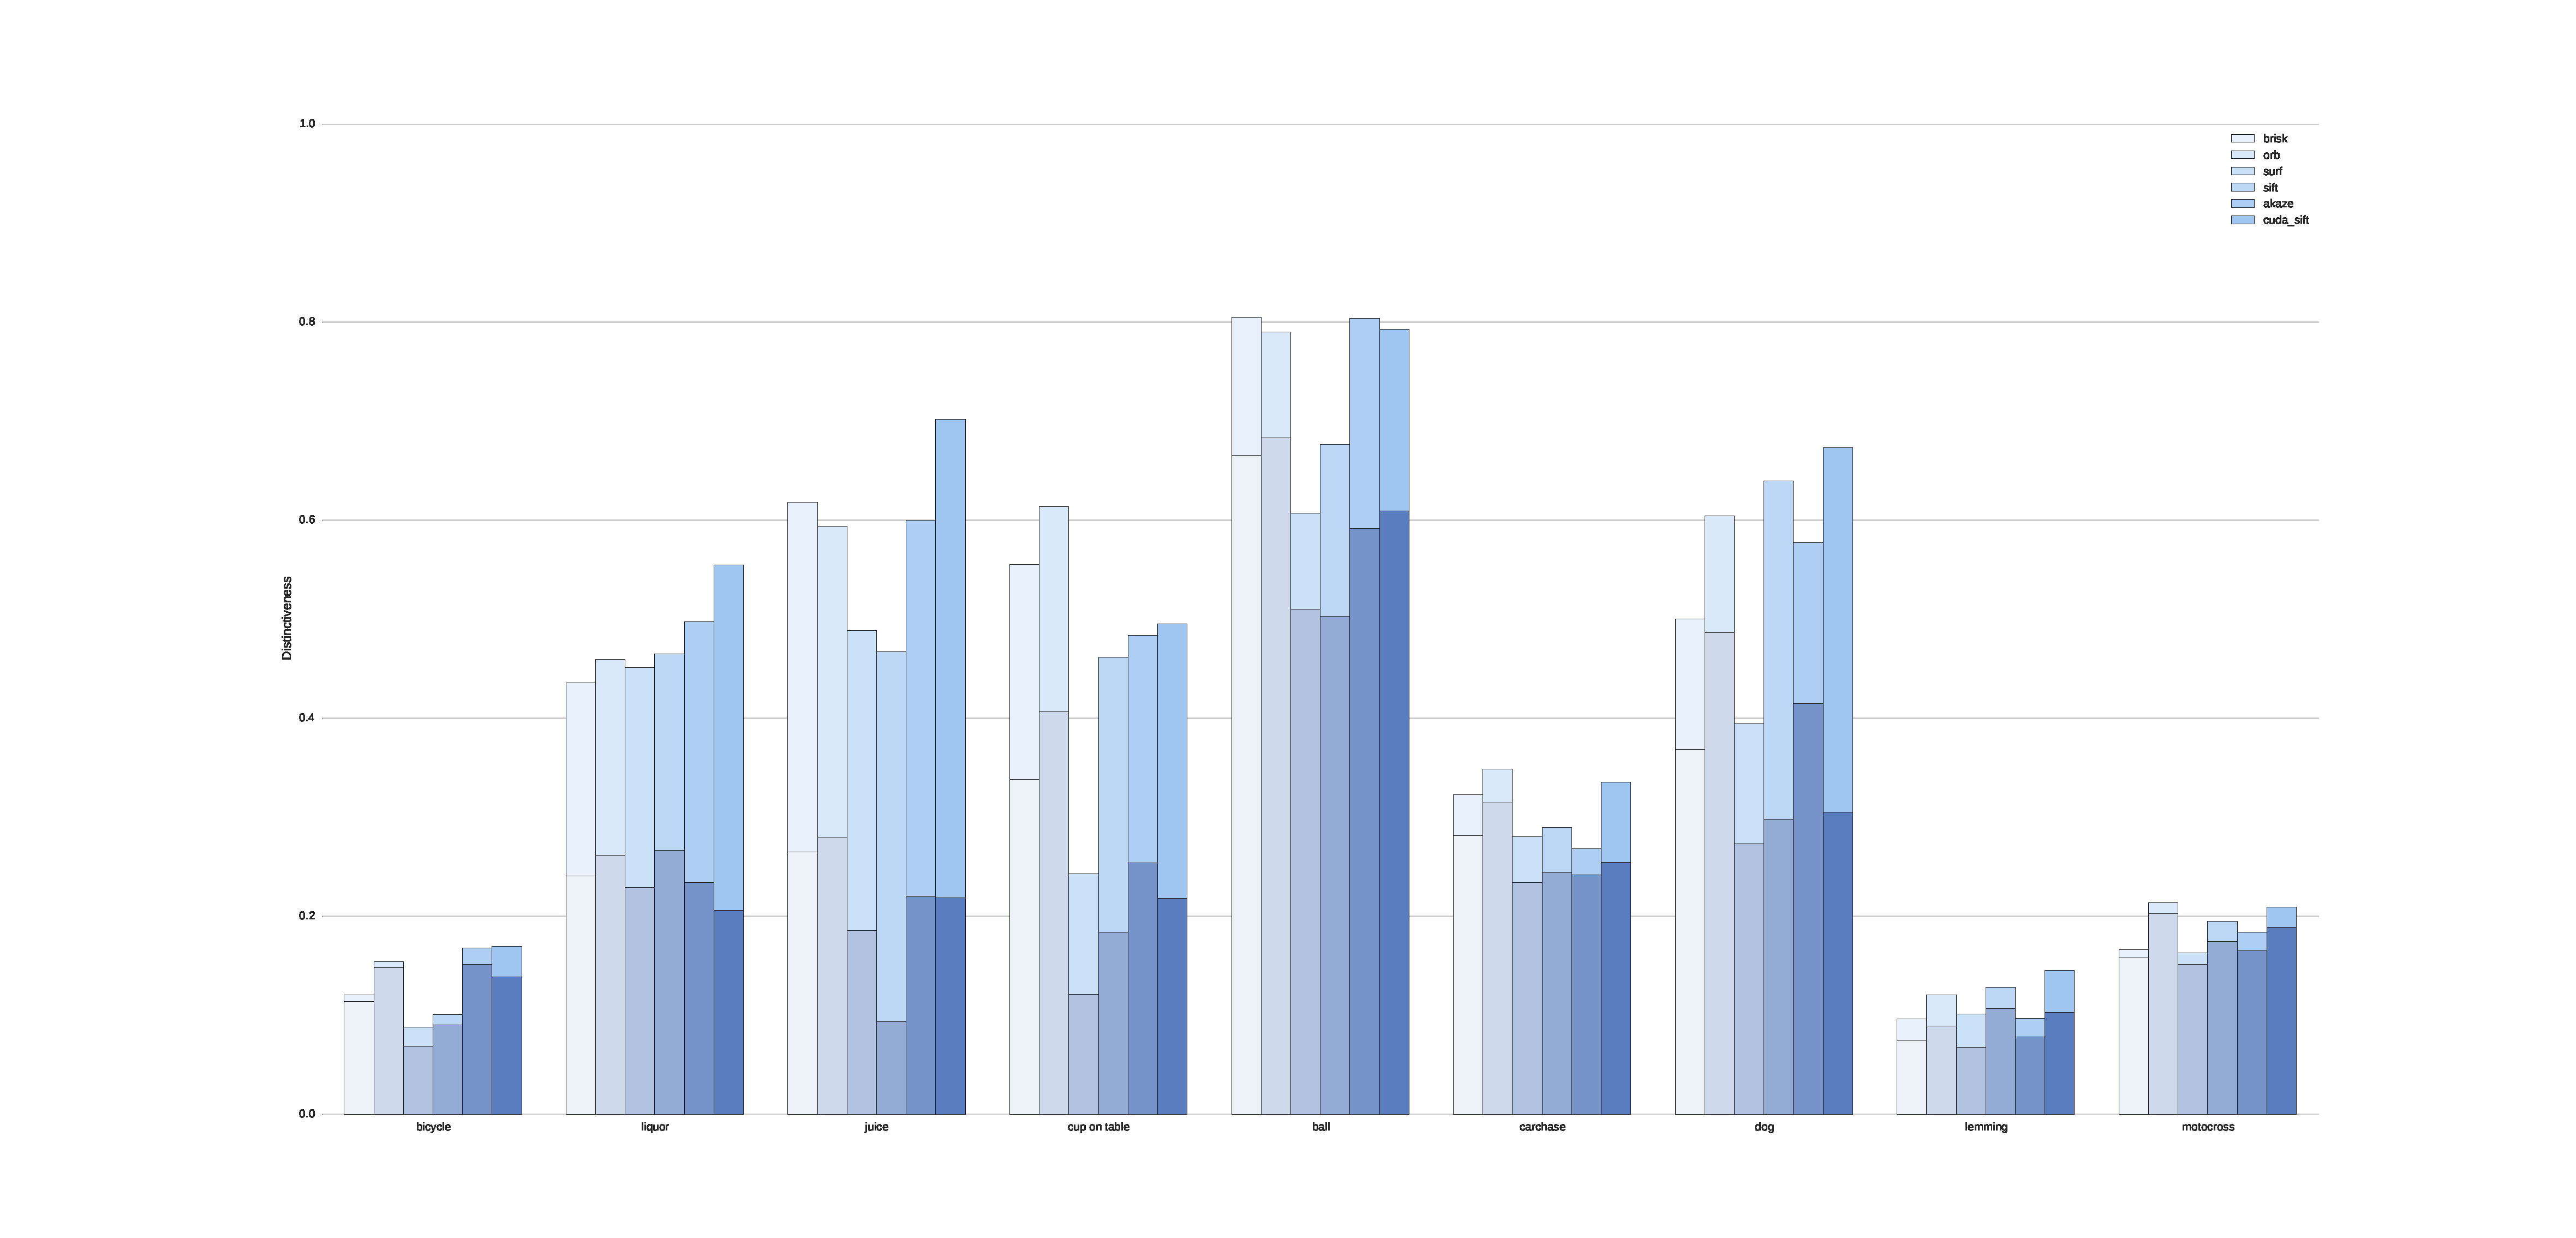
\includegraphics[width=0.98\linewidth]{imgs/distinctivenessTP.pdf}}
%    \vspace{-2mm} 
%	\caption{Examples taken from the dataset showing the ratio of true positives and ambiguous true positives. The lighter color bars show the number of true positives that will actually pass the second best result test.}
%	\label{fig:distinctiveness}
%\end{figure*}

The first aspect was to assess the distinctiveness. Table~\ref{table:tp_ratio} shows the average number of key-points extracted, descriptors belonging to the object to track and the ratio of true positives (TP), false positives (FP) and true positives that pass the second best match ratio check (TTP). 

\begin{table}[!h]
\caption{Average number of feature extracted, object features, true positives and false positives. Every row is normalized by its maximum value.}
\vspace{-2mm} 
\centerline{% 
		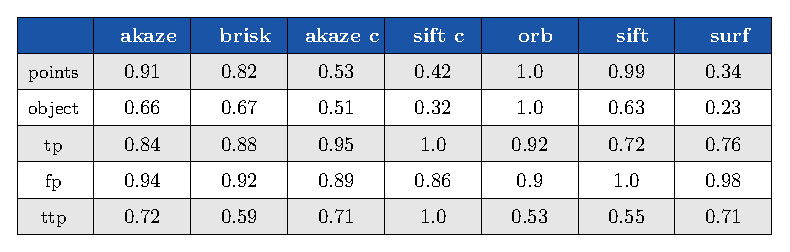
\includegraphics[width=0.98\linewidth]{tables/descriptivness_ratio.pdf}}
    \vspace{-2mm} 
	\label{table:tp_ratio}
\end{table}

It is interesting to notice that BRISK, ORB and SIFT extract a higher number of feature descriptors in general. In particular, BRISK and ORB have a higher number of key-points extracted within the area of the object. However, looking at the average amount of true positives, it can be seen that the best performing descriptors are AKAZE and the implementation of SIFT on the GPU. This is a first indicator of the quality of the descriptors extracted. Moreover, it can be noticed that the true positives are also more distinctive in the case of AKAZE and SIFT since the number of TTP is higher.

\begin{table*}[t]
\caption{Tracking results with low, medium and high accuracy requirements. The high number of key points extracted by ORB or BRISK compensate their weak descriptors. This comes with a cost in performance.} 
\centerline{%
		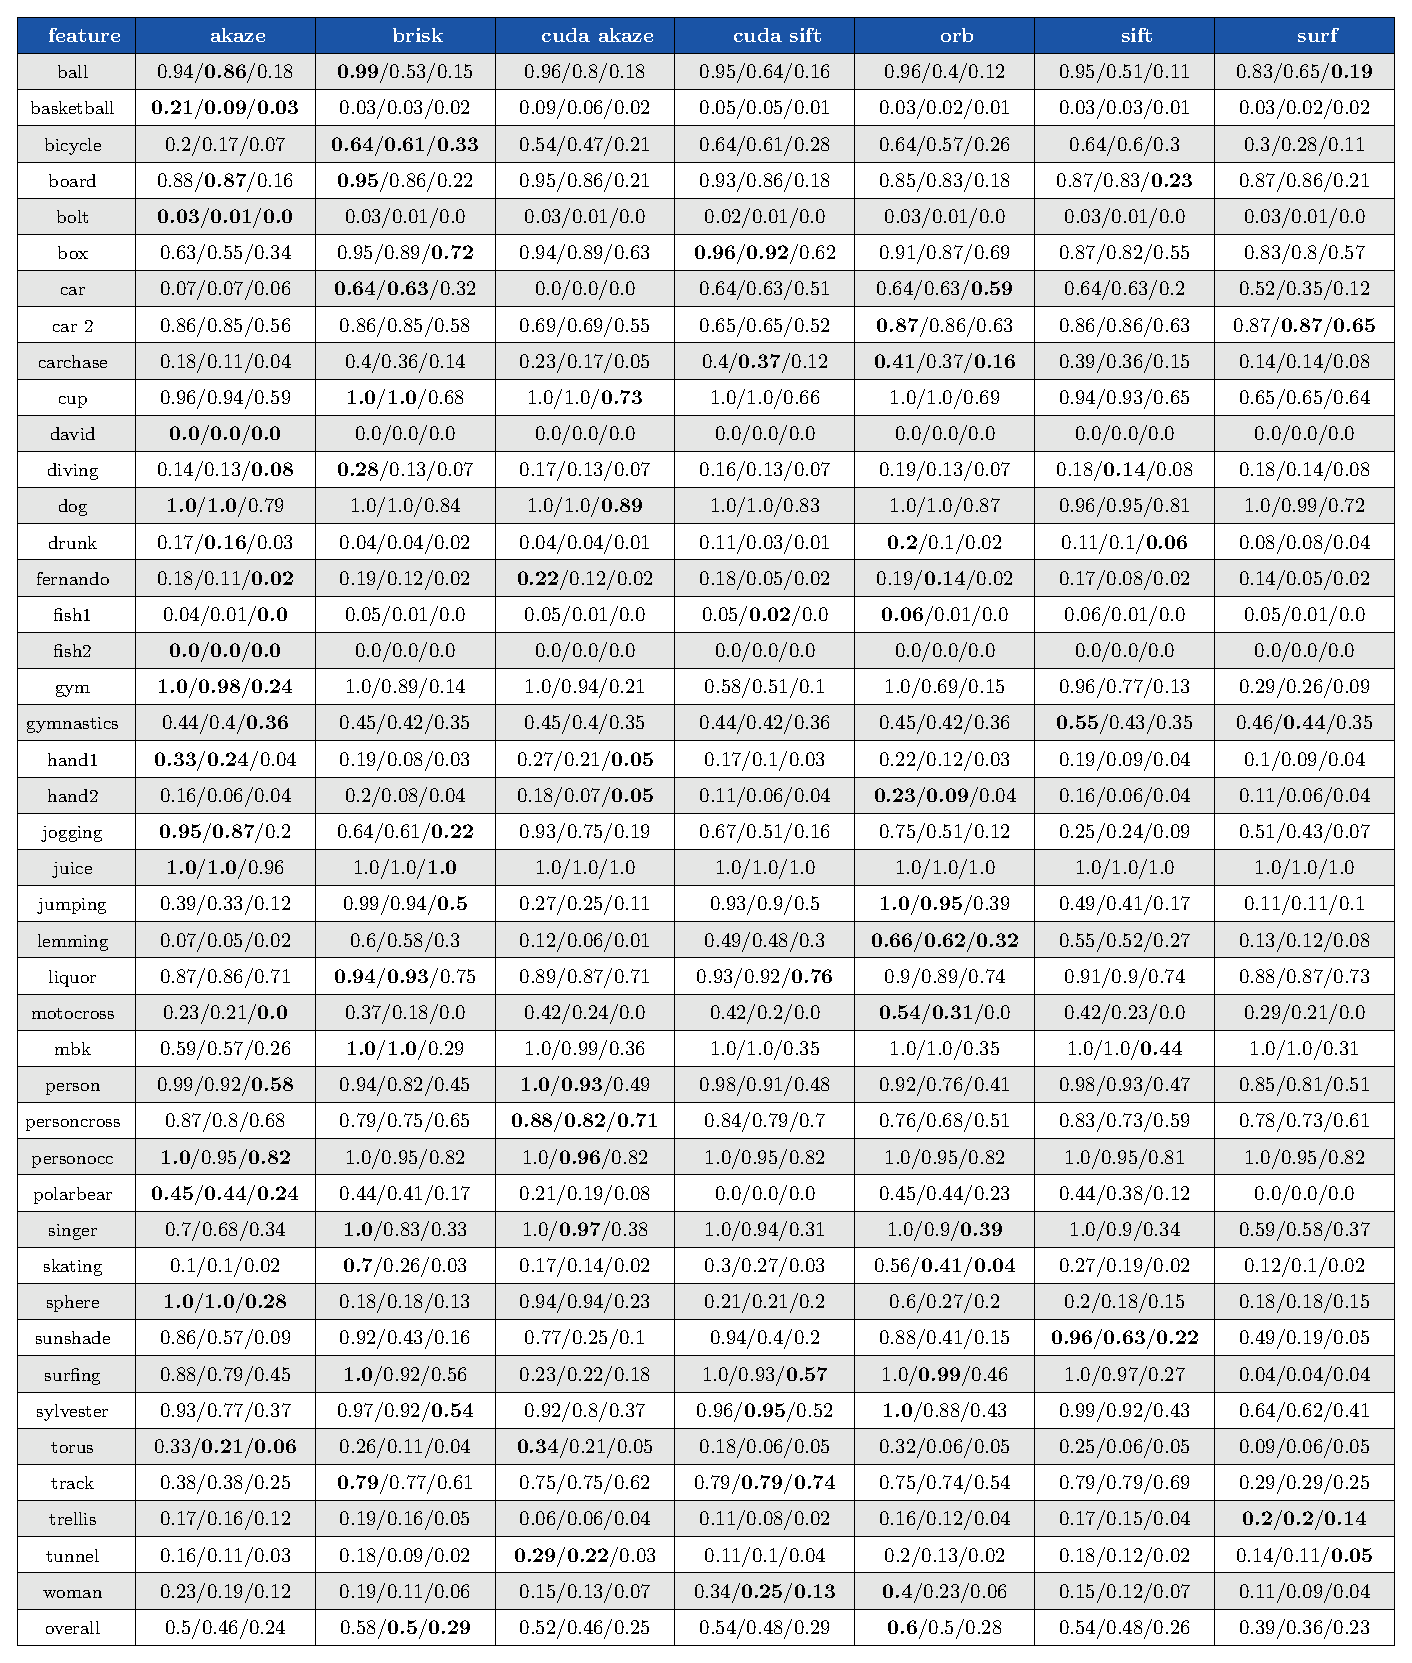
\includegraphics[width=\linewidth]{tables/tracking_precision.pdf}}
		\vspace{8mm}
	\label{table:taccuracy}
\end{table*}


\subsection{Tracking accuracy}

As explained in the previous section, we evaluated the accuracy of the feature descriptors by running our tracker and calculating the overlap measure for low, medium and high accuracy requirements. 
\begin{figure}[!h]
	\vspace{2mm}
\centerline{%
	\subfigure{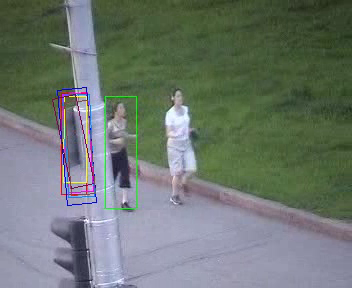
\includegraphics[width=0.48\linewidth]{imgs/results/ex5.png}}
	\subfigure{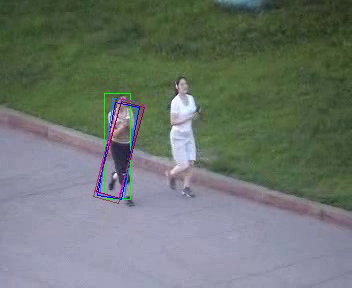
\includegraphics[width=0.48\linewidth]{imgs/results/ex6.png}}}
\caption{Examples showing the behaviour of the feature descriptors upon occlusion. Upon recovery from track loss more descriptive descriptors allow the tracker to recover faster.}
\vspace{-3mm}
\label{fig:tracking_results}
\end{figure}

Table~\ref{table:taccuracy} summarizes tracking results on all the video sequences included in the dataset.  Our experiments show that AKAZE, BRISK, ORB and SIFT have comparable results. It is interesting to note that BRISK and ORB compensate their weak distinctiveness with a higher amount of weak descriptors extracted. A high number of feature points proved to be effective in tracking in the video sequences where the object suffers drastic scale changes and full occlusion, making the recovery after track loss faster, see Fig.~\ref{fig:tracking_results}. We also noticed that AKAZE, more than SIFT, suffers the change in scale. 

\subsection{Tracking performance}

The dataset used for benchmarking includes video sequences of various resolution. Fig.~\ref{fig:speed} shows the average performance of each feature descriptor on the resolutions having the highest number of sequences. 

\begin{figure}[!htb]
	%\vspace{-2mm}
	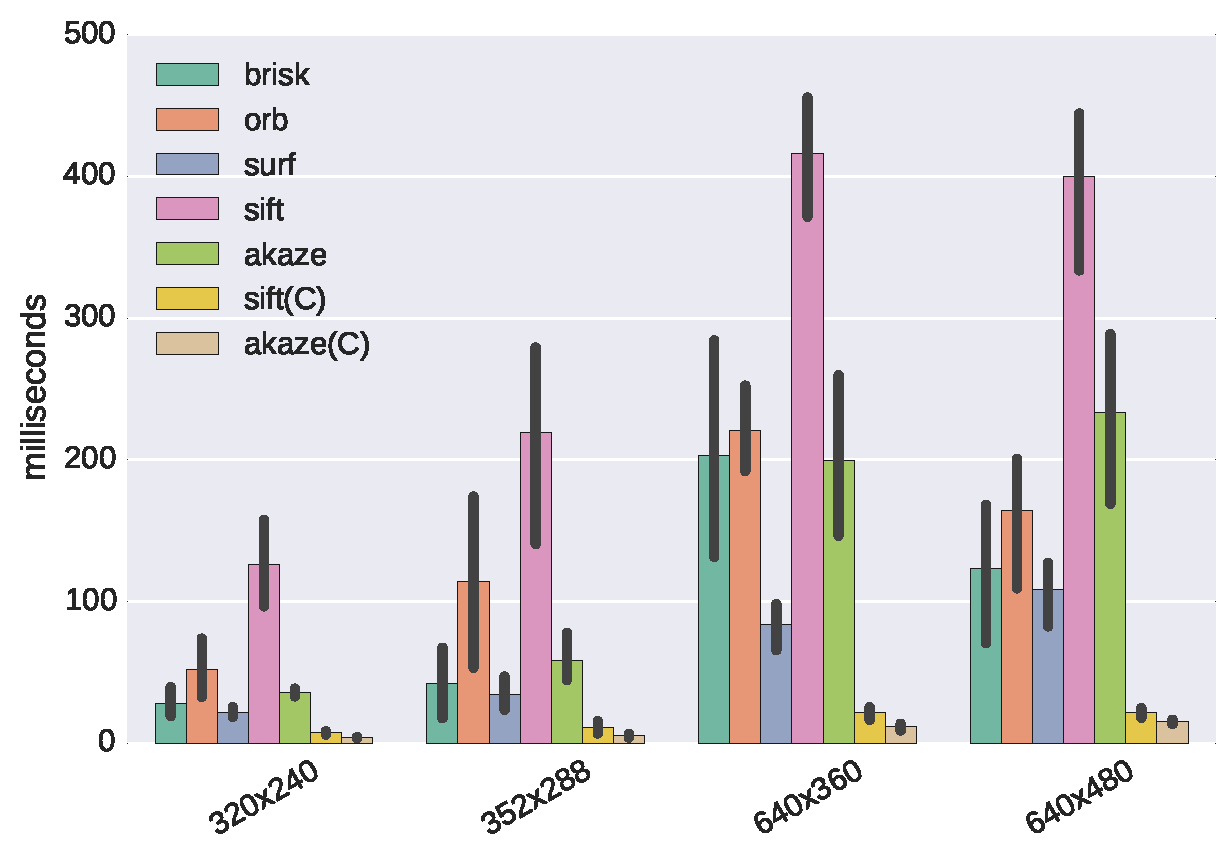
\includegraphics[width=0.95\linewidth]{imgs/tracker_fps_std.pdf}
\vspace{-2.5mm}	
\caption{Average time spent on tracking the object in a single frame: important factors are the resolution and the number of feature descriptors extracted. The variance of the results is a good indication of how much the number of feature descriptors influences the performance. It can be seen that the implementations have a lower variation due to the high level of parallelism. }
\vspace{-2mm}
\label{fig:speed}
\end{figure}

The two most important factors that influence performance are resolution and number of key points extracted. The former influences particularly the detection step when the scale space of descriptors is computed and key-points are detected. The latter influences more the extraction step when feature descriptors are calculated and the matching step. The average performance of each separate step can be seen in Fig.~\ref{fig:speed_b}. One interesting aspect to notice is the variance of the performance in Fig.~\ref{fig:speed}: BRISK, ORB and SIFT have the higher variance while CUDA SIFT and CUDA AKAZE have lower variance. This is also a good indicator of the level of parallelism of the implementation of the descriptor. It is interesting to notice that the computation of the non linear scale space required by AKAZE is not perfectly suited for a GPU architecture since it requires many sequential steps, as a result the key-detector is slower that SIFT. However since the descriptor is binary, its extraction and matching compensate in terms of performance. It is also important to remember that CPU implementations do not exploit the same number of cores, complicating a fair comparison between methods.

\begin{figure}[!htb]
	%\vspace{-2mm}
	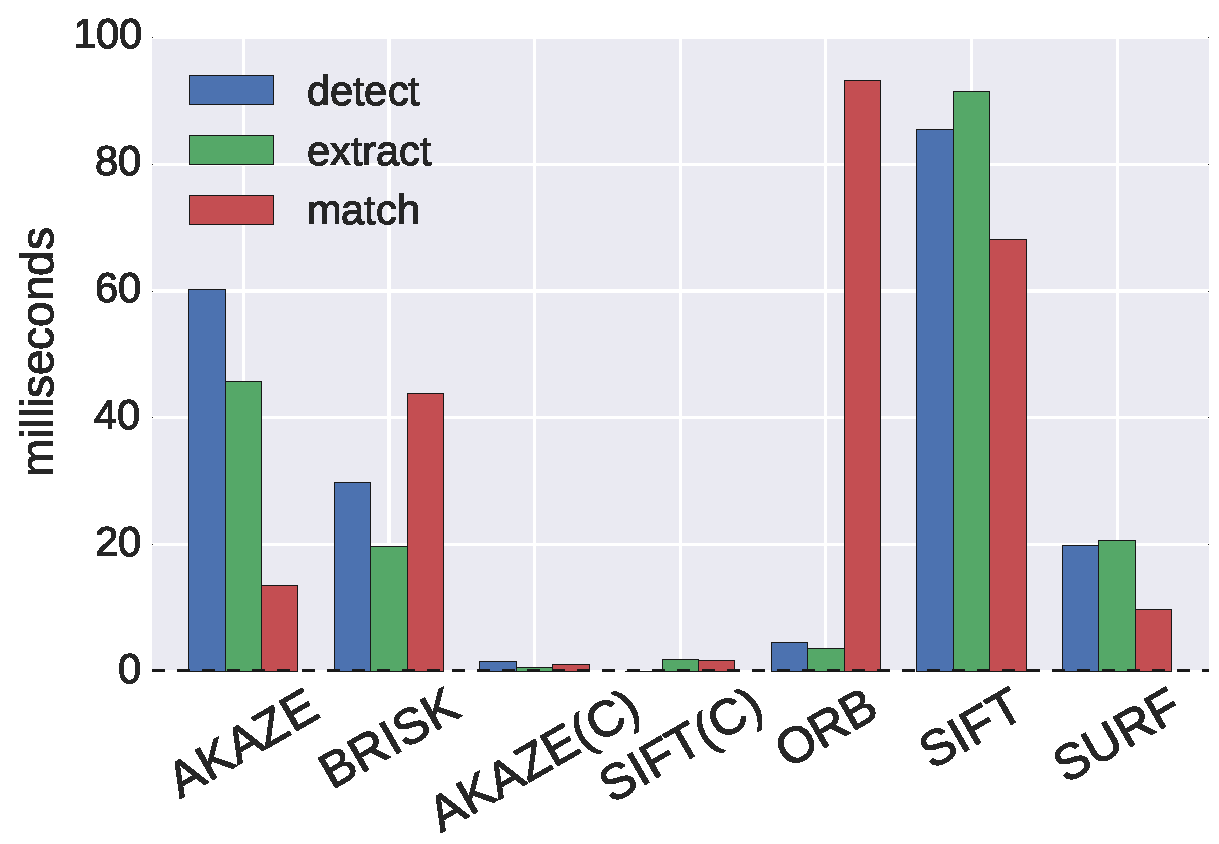
\includegraphics[width=0.95\linewidth]{imgs/performances.pdf}
\vspace{-2.5mm}	
\caption{Performance of the detect, extract and match steps of each feature descriptor.}
\label{fig:speed_b}
\end{figure}

%\begin{table}
%\caption{Average time spent on a single frame by the tracker.}
	%\vspace{-2mm}
%	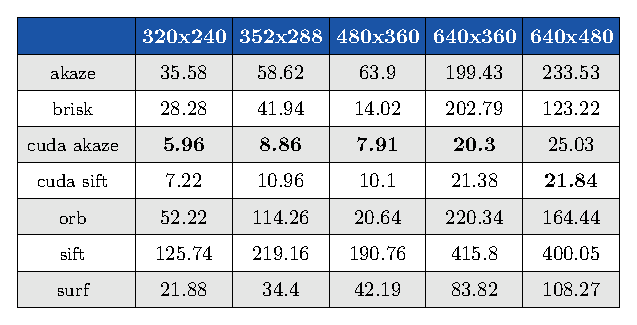
\includegraphics[width=0.95\linewidth]{tables/resolution_times.pdf}
%\vspace{-2.5mm}	
%\label{fig:fps}
%\end{table}

\subsection{Discussion}

Most of the feature descriptors proved to be effective for tracking purposes showing a good precision and performance. This is positive since it makes these suitable for real-time applications. Despite being assessed as somewhat weak in terms of distinctiveness, ORB and BRISK have been proven to be good for real time frameworks. 
However, the trade-off between the distinctiveness and accuracy is not easy to define.
AKAZE and SIFT have been proven to be more distinctive as descriptors but only their implementations on the GPU allow real time performances. 
The most important factors that diversify the results are the characteristics of the video sequences: object transformations, in particular scale, object appearance, light condition and motion blur. AKAZE and SIFT have shown to be more distinctive and effective when the video does not present drastic movements. AKAZE seems to be particularly sensitive to change in scale or blurring, on the other hand it has higher performance on low textured objects and people, still in sequences where the tracked object keep a constant distance from the camera as in Fig.~\ref{fig:tracking_comparison}.
Moreover, we noticed that the matching rate of all features drop consistently upon fast movements of the camera as we discussed in \cite{pieropan15}. However, the performance of weak feature descriptors such as BRISK or ORB seems to be less sensitive to this kind of noise as in Fig.~\ref{fig:tracking_comparison}. 

\begin{figure}[!htb]
	\vspace{2mm}
\centerline{%
	\subfigure[scale]{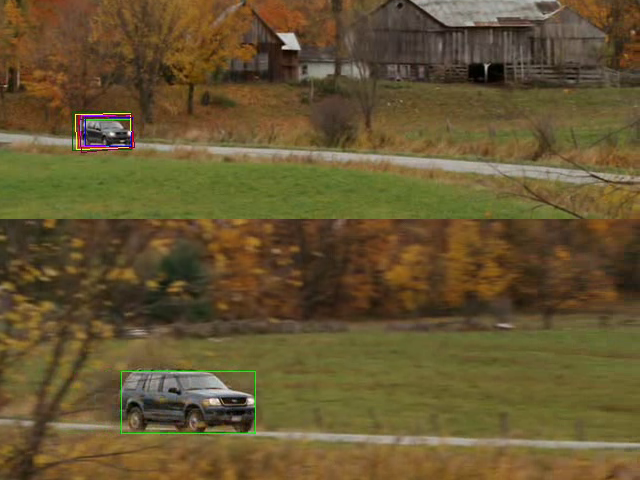
\includegraphics[width=0.33\linewidth]{imgs/limitations/scale.png}\label{fig:tra}}
	\subfigure[light]{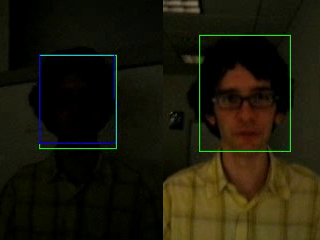
\includegraphics[width=0.33\linewidth]{imgs/limitations/light.png}\label{fig:trb}}
	\subfigure[multi-instance]{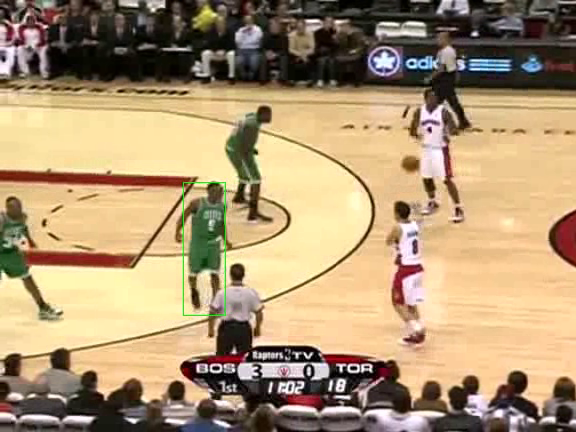
\includegraphics[width=0.33\linewidth]{imgs/limitations/basket.png}\label{fig:trc}}}
	\vspace{-2mm}
\caption{Examples showing the main problems that feature descriptors cannot address. }
\label{fig:tracking_results_scale}
\end{figure} 


There are still some issue that need to be addressed in relation to achieving a robust tracking system. First, even if many descriptors are invariant to scale or rotation, we noticed that this does
not hold for drastic changes like in Fig.~\ref{fig:tra}. One possible solution is to extract features from appearances of the object generated through synthetic transformations. It has been shown by Morel \cite{morel2009} that this technique improves the matching performance of SIFT descriptor.  
Second, feature descriptors are sensitive to light conditions, see Fig.~\ref{fig:trb}. This is particularly relevant for robotics applications since the interaction of a robotic platform with a target object may occlude the light source. Third, the common matching approach to detect an object or compute the transformation between images \cite{mikolajczyk05} does not work in the presence of multiple targets with similar appearance. This is the case shown in Fig.\ref{fig:trc} where more players have the same outfit.



\begin{figure*}[!htb]
	\vspace{2mm}
\centerline{%
	\subfigure[Crossing: constant distance from camera, target often occluded.]{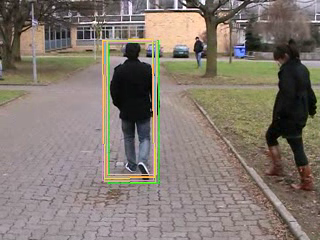
\includegraphics[width=0.24\linewidth]{imgs/comparison/occ1.png}
			   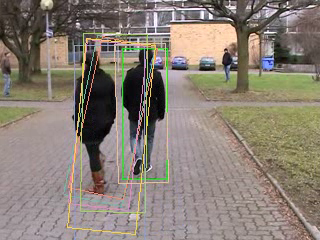
\includegraphics[width=0.24\linewidth]{imgs/comparison/occ2.png}
			   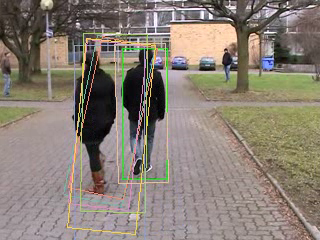
\includegraphics[width=0.24\linewidth]{imgs/comparison/occ2.png}
			   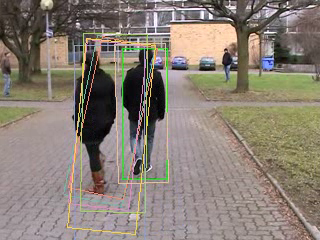
\includegraphics[width=0.24\linewidth]{imgs/comparison/occ2.png}}
			   \label{fig:crossing}}
	\vspace{-2mm}
\centerline{%
	\subfigure[Jumping: high motion blur.]{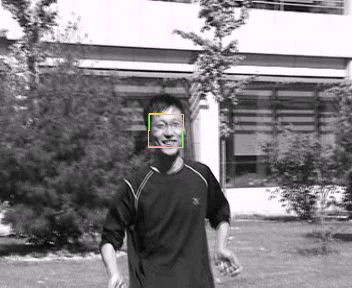
\includegraphics[width=0.24\linewidth,trim={0, 0 0 2cm},clip]{imgs/comparison/blur1.png}
	           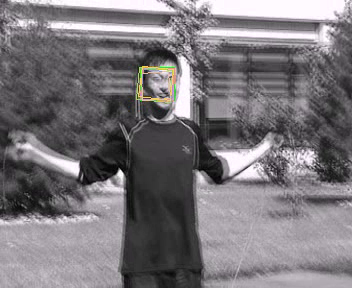
\includegraphics[width=0.24\linewidth,trim={0, 0 0 2cm},clip]{imgs/comparison/blur2.png}
			   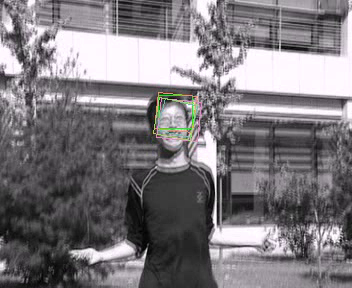
\includegraphics[width=0.24\linewidth,trim={0, 0 0 2cm},clip]{imgs/comparison/blur3.png}
	           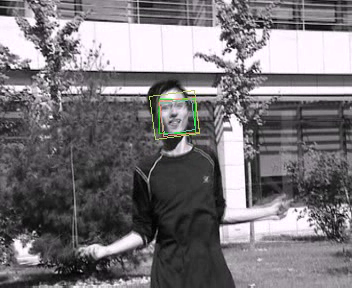
\includegraphics[width=0.24\linewidth,trim={0, 0 0 2cm},clip]{imgs/comparison/blur4.png}}
	           \label{fig:jumping}}
	           \centerline{%
\subfigure[Skating: motion blur, scale and light change.]{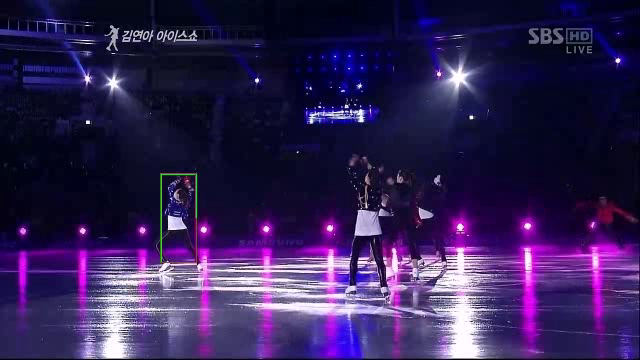
\includegraphics[width=0.24\linewidth]{imgs/comparison/skating1.png}
	           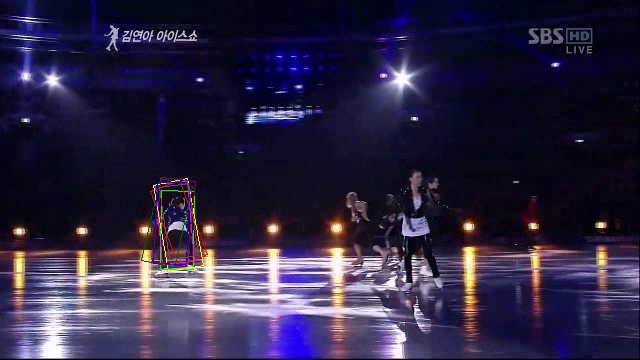
\includegraphics[width=0.24\linewidth]{imgs/comparison/skating2.png}
	           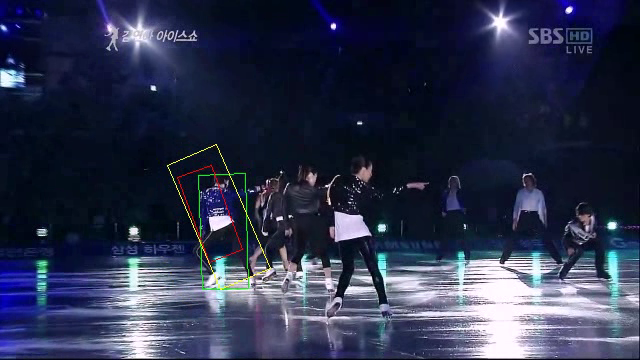
\includegraphics[width=0.24\linewidth]{imgs/comparison/skating3.png}
	           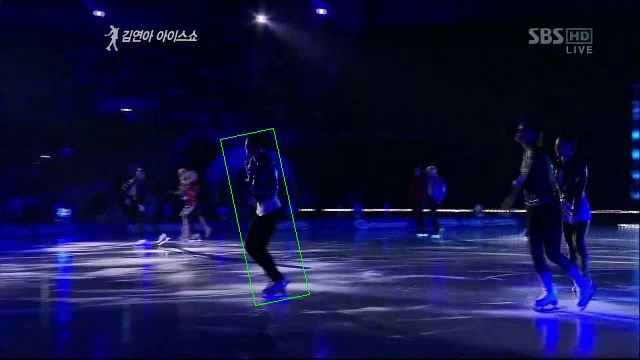
\includegraphics[width=0.24\linewidth]{imgs/comparison/skating4.png}}
	           \label{fig:skating}}
\caption{A few example where the precision of the descriptors differs consistently. In sequence~(a) AKAZE the camera keeps the a constant distance from the target who is often occluded by other people. SIFT and AKAZE performs better in this scenario. In sequence~(b) the target is often blurred due to high motion, ORB and BRISK have the best precision in such as scenario. Sequence~(c) is one of the most challenging, it contains scale and light changes and motion blur. BRISK and ORB have higher accuracy however on light changes all the descriptors lose the target.}
\vspace{-3mm}
\label{fig:tracking_comparison}
\end{figure*}





